\begin{figure}
  \centering
  \begin{subfigure}{.45\textwidth}
    \resizebox{\textwidth}{!}{
    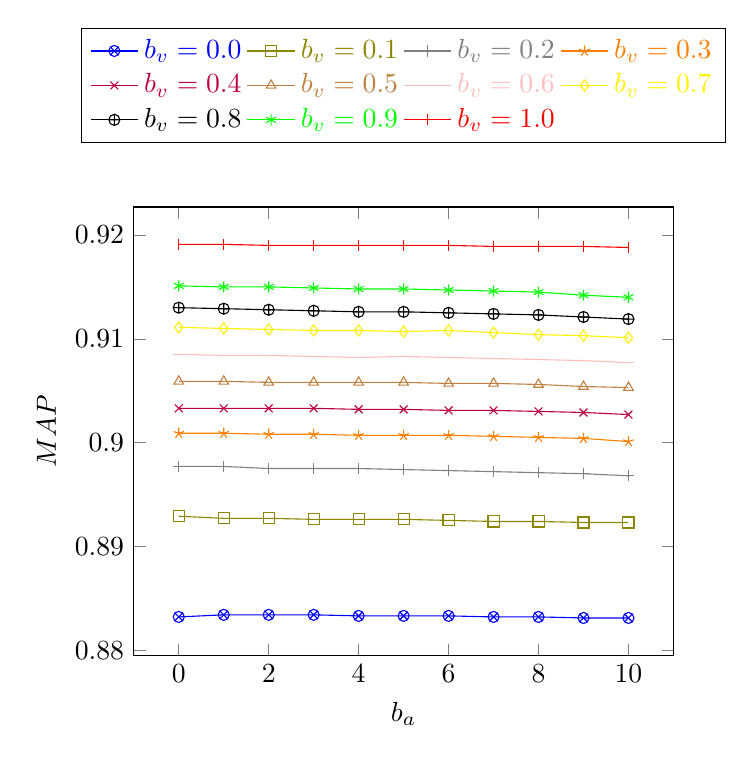
\begin{tikzpicture}
       \begin{axis}[
         xlabel=$b_a$,
         ylabel=$MAP$,
         legend style={at={(0.5, 1.4)}, anchor=north, legend columns=4},
         legend entries={
           [blue]$b_v = 0.0$,
           [olive]$b_v = 0.1$,
           [gray]$b_v = 0.2$,
           [orange]$b_v = 0.3$,
           [purple]$b_v = 0.4$,
           [brown]$b_v = 0.5$,
           [pink]$b_v = 0.6$,
           [yellow]$b_v = 0.7$,
           [black]$b_v = 0.8$,
           [green]$b_v = 0.9$,
           [red]$b_v = 1.0$
         }
       ]
           \addplot[mark=otimes, style=solid, color=blue] coordinates { (0, 0.8832) (1, 0.8834) (2, 0.8834) (3, 0.8834) (4, 0.8833) (5, 0.8833) (6, 0.8833) (7, 0.8832) (8, 0.8832) (9, 0.8831) (10, 0.8831) };
           \addplot[mark=square, style=solid, color=olive] coordinates { (0, 0.8929) (1, 0.8927) (2, 0.8927) (3, 0.8926) (4, 0.8926) (5, 0.8926) (6, 0.8925) (7, 0.8924) (8, 0.8924) (9, 0.8923) (10, 0.8923) };
           \addplot[mark=+, style=solid, color=gray] coordinates { (0, 0.8977) (1, 0.8977) (2, 0.8975) (3, 0.8975) (4, 0.8975) (5, 0.8974) (6, 0.8973) (7, 0.8972) (8, 0.8971) (9, 0.8970) (10, 0.8968) };
           \addplot[mark=star, style=solid, color=orange] coordinates { (0, 0.9009) (1, 0.9009) (2, 0.9008) (3, 0.9008) (4, 0.9007) (5, 0.9007) (6, 0.9007) (7, 0.9006) (8, 0.9005) (9, 0.9004) (10, 0.9001) };
           \addplot[mark=x, style=solid, color=purple] coordinates { (0, 0.9033) (1, 0.9033) (2, 0.9033) (3, 0.9033) (4, 0.9032) (5, 0.9032) (6, 0.9031) (7, 0.9031) (8, 0.9030) (9, 0.9029) (10, 0.9027) };
           \addplot[mark=triangle, style=solid, color=brown] coordinates { (0, 0.9059) (1, 0.9059) (2, 0.9058) (3, 0.9058) (4, 0.9058) (5, 0.9058) (6, 0.9057) (7, 0.9057) (8, 0.9056) (9, 0.9054) (10, 0.9053) };
           \addplot[mark=-, style=solid, color=pink] coordinates { (0, 0.9085) (1, 0.9084) (2, 0.9084) (3, 0.9083) (4, 0.9082) (5, 0.9083) (6, 0.9082) (7, 0.9081) (8, 0.9080) (9, 0.9079) (10, 0.9077) };
           \addplot[mark=diamond, style=solid, color=yellow] coordinates { (0, 0.9111) (1, 0.9110) (2, 0.9109) (3, 0.9108) (4, 0.9108) (5, 0.9107) (6, 0.9108) (7, 0.9106) (8, 0.9104) (9, 0.9103) (10, 0.9101) };
           \addplot[mark=oplus, style=solid, color=black] coordinates { (0, 0.9130) (1, 0.9129) (2, 0.9128) (3, 0.9127) (4, 0.9126) (5, 0.9126) (6, 0.9125) (7, 0.9124) (8, 0.9123) (9, 0.9121) (10, 0.9119) };
           \addplot[mark=asterisk, style=solid, color=green] coordinates { (0, 0.9151) (1, 0.9150) (2, 0.9150) (3, 0.9149) (4, 0.9148) (5, 0.9148) (6, 0.9147) (7, 0.9146) (8, 0.9145) (9, 0.9142) (10, 0.9140) };
           \addplot[mark=|, style=solid, color=red] coordinates { (0, 0.9191) (1, 0.9191) (2, 0.9190) (3, 0.9190) (4, 0.9190) (5, 0.9190) (6, 0.9190) (7, 0.9189) (8, 0.9189) (9, 0.9189) (10, 0.9188) };
       \end{axis}
    \end{tikzpicture}
    }
    \caption{Average over simple graphs}
    \label{fig:summary-ranking-norm-simple}
  \end{subfigure}
  \quad
  \begin{subfigure}{.45\textwidth}
    \resizebox{\textwidth}{!}{
    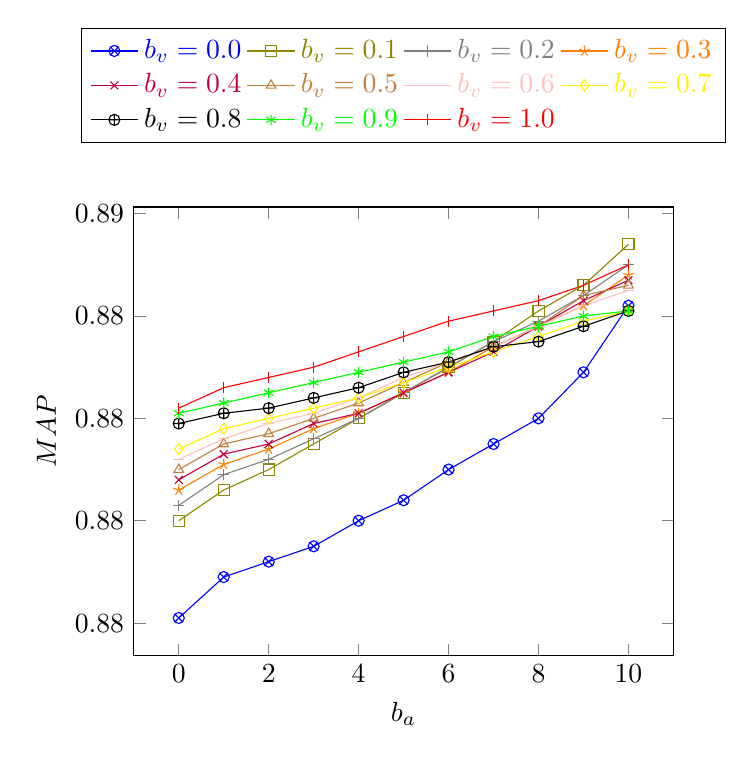
\begin{tikzpicture}
       \begin{axis}[
         xlabel=$b_a$,
         ylabel=$MAP$,
         legend style={at={(0.5, 1.4)}, anchor=north, legend columns=4},
         legend entries={
           [blue]$b_v = 0.0$,
           [olive]$b_v = 0.1$,
           [gray]$b_v = 0.2$,
           [orange]$b_v = 0.3$,
           [purple]$b_v = 0.4$,
           [brown]$b_v = 0.5$,
           [pink]$b_v = 0.6$,
           [yellow]$b_v = 0.7$,
           [black]$b_v = 0.8$,
           [green]$b_v = 0.9$,
           [red]$b_v = 1.0$
         }
       ]
           \addplot[mark=otimes, style=solid, color=blue] coordinates { (0, 0.8781) (1, 0.8789) (2, 0.8792) (3, 0.8795) (4, 0.8800) (5, 0.8804) (6, 0.8810) (7, 0.8815) (8, 0.8820) (9, 0.8829) (10, 0.8842) };
           \addplot[mark=square, style=solid, color=olive] coordinates { (0, 0.8800) (1, 0.8806) (2, 0.8810) (3, 0.8815) (4, 0.8820) (5, 0.8825) (6, 0.8830) (7, 0.8835) (8, 0.8841) (9, 0.8846) (10, 0.8854) };
           \addplot[mark=+, style=solid, color=gray] coordinates { (0, 0.8803) (1, 0.8809) (2, 0.8812) (3, 0.8816) (4, 0.8820) (5, 0.8825) (6, 0.8830) (7, 0.8835) (8, 0.8839) (9, 0.8844) (10, 0.8850) };
           \addplot[mark=star, style=solid, color=orange] coordinates { (0, 0.8806) (1, 0.8811) (2, 0.8814) (3, 0.8818) (4, 0.8821) (5, 0.8825) (6, 0.8829) (7, 0.8834) (8, 0.8838) (9, 0.8842) (10, 0.8848) };
           \addplot[mark=x, style=solid, color=purple] coordinates { (0, 0.8808) (1, 0.8813) (2, 0.8815) (3, 0.8819) (4, 0.8821) (5, 0.8825) (6, 0.8829) (7, 0.8833) (8, 0.8838) (9, 0.8843) (10, 0.8847) };
           \addplot[mark=triangle, style=solid, color=brown] coordinates { (0, 0.8810) (1, 0.8815) (2, 0.8817) (3, 0.8820) (4, 0.8823) (5, 0.8827) (6, 0.8831) (7, 0.8834) (8, 0.8838) (9, 0.8844) (10, 0.8846) };
           \addplot[mark=-, style=solid, color=pink] coordinates { (0, 0.8812) (1, 0.8816) (2, 0.8819) (3, 0.8821) (4, 0.8824) (5, 0.8828) (6, 0.8831) (7, 0.8834) (8, 0.8838) (9, 0.8842) (10, 0.8845) };
           \addplot[mark=diamond, style=solid, color=yellow] coordinates { (0, 0.8814) (1, 0.8818) (2, 0.8820) (3, 0.8822) (4, 0.8824) (5, 0.8827) (6, 0.8830) (7, 0.8833) (8, 0.8836) (9, 0.8839) (10, 0.8841) };
           \addplot[mark=oplus, style=solid, color=black] coordinates { (0, 0.8819) (1, 0.8821) (2, 0.8822) (3, 0.8824) (4, 0.8826) (5, 0.8829) (6, 0.8831) (7, 0.8834) (8, 0.8835) (9, 0.8838) (10, 0.8841) };
           \addplot[mark=asterisk, style=solid, color=green] coordinates { (0, 0.8821) (1, 0.8823) (2, 0.8825) (3, 0.8827) (4, 0.8829) (5, 0.8831) (6, 0.8833) (7, 0.8836) (8, 0.8838) (9, 0.8840) (10, 0.8841) };
           \addplot[mark=|, style=solid, color=red] coordinates { (0, 0.8822) (1, 0.8826) (2, 0.8828) (3, 0.8830) (4, 0.8833) (5, 0.8836) (6, 0.8839) (7, 0.8841) (8, 0.8843) (9, 0.8846) (10, 0.8850) };
       \end{axis}
    \end{tikzpicture}
    }
    \caption{Average over complex graphs}
    \label{fig:summary-ranking-norm-complex}
  \end{subfigure}
  \caption{MF normalisation parameters over simple and complex graphs}
  \label{fig:summary-ranking-norm}
\end{figure}
